\documentclass[11pt]{article}
\usepackage[top=1in, bottom=1in, left=1in, right=1in]{geometry}
\usepackage{listings}
\usepackage{setspace}
\usepackage{color}
\usepackage{graphicx}



\renewcommand{\baselinestretch}{1.4}
\setlength{\parskip}{0.8em}
 
\definecolor{codegreen}{rgb}{0,0.6,0}
\definecolor{codegray}{rgb}{0.5,0.5,0.5}
\definecolor{codepurple}{rgb}{0.58,0,0.82}
\definecolor{backcolour}{rgb}{0.95,0.95,0.92}

\lstdefinestyle{codestyle}{
	language=Java,
    backgroundcolor=\color{backcolour},   
    commentstyle=\color{codegreen},
    keywordstyle=\color{magenta},
    numberstyle=\tiny\color{codegray},
    stringstyle=\color{codepurple},
    basicstyle=\footnotesize\ttfamily,
    breakatwhitespace=false,         
    breaklines=true,                 
    captionpos=b,                    
    keepspaces=true,                 
    numbers=left,                    
    numbersep=5pt,                  
    showspaces=false,                
    showstringspaces=false,
    showtabs=false,                  
    tabsize=2
}
\lstset{style=codestyle}

\newcommand{\quotes}[1]{``#1"}

\begin{document}

\begin{center}
\textbf{ECE 458: Engineering Software For Maintainability \\
Senior Design Course\\
Spring 2015\\[0.2in]}
Evolution 2 Analysis\\
Brian Bolze, Jeff Day, Henrique Rusca, Wes Koorbusch
\end{center}

\singlespacing
\tableofcontents

% Writen Analysis (25%) Along with every software deliverable, you will turn in a written docu- ment which will cover two main points:

% 1. A retrospective on how your previous design choices impacted your work to meet the current set of requirements. This section should analyze not only where your good design choices made things easy, but also where your bad design choices made things hard. For both of these points, you should analyze how/why these design choices helped or hindered you. For bad design choices, you should discuss what you might have done differently in the past to avoid the problem this time around.

% 2. An evaluation of your current design, with an analysis of its strengths and weaknesses going forwards. This section should justify your current design choices, explaining why you think they will be beneficial to you in the long run. If you recognize weaknesses in your current design, you should discuss them—including an explanation of why they are there, and how you plan to fix them in future submissions.

% These documents should not only deep analysis of the strengths and weaknesses of your design choice, but also be well written. Ideally, the retrospective section of submission N would connect back to the forward-looking analysis of submission N-1 (i.e., Did things you think would be beneficial actually end up helping you? Did the weaknesses you identified come back to bite you? Did you fix your weaknesses this time around?).

\pagebreak

\section{Previous Design Analysis}

Considering our groups general inexperience with Rails, we as a group were generally very happy with how our previous design choices impacted our ability to fulfill Evolution 2 requirements.  One key design feature that we created in our model that made some things very simple for us in this evolution was the idea of a subscription.  At the time, we believed that having a user subscribe to a specific event would make notifications, requests, and updates easier to add in the future.  This particularly helped with things like email reminders.  A second design decision that we unfortunately unable to implement in Evolution 1 but had always planned to include was a visibility model object.  There was a significant discussion over whether or not visibility should simply be an aspect of the event field or whether it should have its own entire definition.  The fact that we planned to have it as a distinct definition in our design made it easier to incorporate the ability to see events or not depending on user choices to requests and invites.

One specific area where our design was poor was with repeating events.  We thought the implementation would be relatively simple: make copies of a single event at some defined period.  However, there are a lot of adjustments that need to be made when editing a repeating event.  Initially, we attempted to make a simple encoding of a single number to the days of a week that an event could be repeated and also the period that it would be repeated.  We then realized, it was very difficult to do math with regards to a calendar with integers that represent days of the week.  As is clear in our Evolution 2 implementation, we refactored our design with regards to repeating events in order to make it more robust and flexible.

\section{Current Design Evaluation}

The design of our code improved significantly since evolution 1. After actually taking time to learn what the rails framework provides us, we were able to write cleaner and more efficient code.

\subsection{Views}

For views, Rails provides the use of partials, helpers, assets, and layouts. These features all come together to allow the developer to create a powerful interface. Rails motto of not repeating yourself allows for efficient interface implementation with a great deal of reusable code.

Layouts can be considered the beginning and end of the html file rendered on screen. With them we are able to render the navigation bar along with any error and notification that comes from an action on the application, since this view code wraps all the rest. On the body of the layout structure, the file yields to the corresponding html file that should be rendered on thee session. Within an html view, we can render several partials, which are basically the opposite of the layout. Instead of wrapping the html file, it is embedded in it. Therefore, we are able to render any piece of html.erb (embedded ruby) code within the html file. This proves to be extremely useful for generating forms. For example, the forms for generating and editing a to-do (how we called PUD event) should have the same fields with the exception of header information and the method called on the controller upon the form submission. Another good use of partials is on the events index page. We have added a new visualization through a list of events and segregated them according to visibility. It would consume a lot of code to rewrite the layout for each event every time. Therefore, for each section of visibility, a new partial is rendered because the event information is the same. Helpers work in a similar way that it allows certain methods to be called from views to perform a certain tasks. In our code, for instance, we call a helper to render an error message in case an error carried from the previous page.

Besides layouts and partials, it is important to notice that embedded ruby files allow us to insert ruby code to create dynamic html files. For instance, we can perform a for loop to iterate over the current events and display their information. Also, Rails provides frameworks to generate forms that provides checkboxes, selections, text fields, date time selections, among other things to later perform mass assignment on the controller, preventing the tedious creation of setting each parameter of an object upon creation or update.

Assets are another important cog for a Rails application. All the js, css, and images are included within the assets folder. Rails make use of asset pipelining to precompile all the assets into a single optimized file so the browser can cache it and not make any further requests. The js in the application is used for popup forms and calendar presentation, while the css is, obviously, used for styling.

\subsection{Controllers}

Rails emphasizes how controllers should be kept with a minimum amount of work. Controllers are basically responsible for extracting the variables that the view will use and redirect the browser based on user action and input condition. Also, bear in mind that complex queries for the extraction of the view’s variables are all moved to the models and placed into methods. The controllers of the application perform their function as demanded however Rails does not fail to warn that the implementation practices are not perfect. Sometimes a controller has to handle more than one model at once. For instance, to created a requested event, the controller should create the event itself, a request\_map, and the requests to be sent to the corresponding users. Nevertheless, we try to keep that logic to a minimum by letting the request\_map take the responsibility of creating its own requests by just passing the ids of the users.

Another important point to notice is that Rails recommends that max amount of shared variables between the controller and the view is constrained to two. However, in some cases this is simply not possible. For instance, the events controller segregates arrays of events by visibility for presentation. It is better to extract and separate each type of event into a different array rather than letting the view make difficult queries and figure where to place the next event on the iteration.

\subsection{Models}

Rails provides a solid framework for models to know where they stand. Rails make use of active records pattern to make a model communicate directly with its database counterpart. Also, ActiveRecords on rails offer validation calls to ensure the data inputted is exactly according to the developer’s conditions. If it is an integer, we can define a minimum and a maximum, if it is a string, we can constrain the length and so on. Therefore, we make use of those validations to ensure there are no surprises while retrieving data.

ActiveRecords allow to define a relation between themselves and other ActiveRecords on the database as long as the have the right column name for it. But Rails not only provides a relationship for one-to-many, one-to-one, and many-to-many, but also provides a through relation. It allows an ActiveRecord to reference another one through an intermediary table on the database. This design eases the use of complex queries and simplifies the code greatly upon implementation. For instance, Events can refer directly to their subscribers (Users) without us writing any code to fetch data from the ‘subscriptions’ table. The joins are made automatically. Another example is the groups table, which can access its members (also Users) directly without retrieving membership models.

A very important part of active records are their callbacks. It is possible do define a method to be called before or after any validation, creation, update, or deletion. These callbacks are fundamental for the cohesion of the database and are a great asset towards design. Methods and configuration can be called automatically over active records without the intervention of controllers. For instance, a To-Do verifies the next time it should be scheduled before creation in case it is recurrent, and reschedules itself if needed before an update (i.e. marked as done). For To-Do allocated events, they verify that their duration is a minimum of 15 minutes before validation and fetches the next to-do based on priority after creation. Finally, a reminder takes care of scheduling its notification task upon creation and unscheduling the task upon destruction to avoid emails of non-existent events.

Last important point of ActiveRecords are dependencies. We are able to specify the dependencies of relation between ActiveRecords and how the deletion of one should affect its related tables. Therefore, we are able to cascade deletions and get rid of potential memory leaks in the database without much trouble. For instance, if a user is deleted, it consequently deletes its created events, that deletes its related request map and requests, to-do items, and subscriptions. To-dos and subscriptions in turn destroy their respective reminders, which get unscheduled before destruction. Therefore, one could argue that the database has a considerably cohesive structure.

\subsection{Database}

The design of the database changed drastically since evolution 1. It got much more complex and with the help of active records callbacks and dependencies, it becomes self-maintainable in many points. Each ActiveRecord has its corresponding table and relations. Those are:

\begin{figure}[H]
\centering
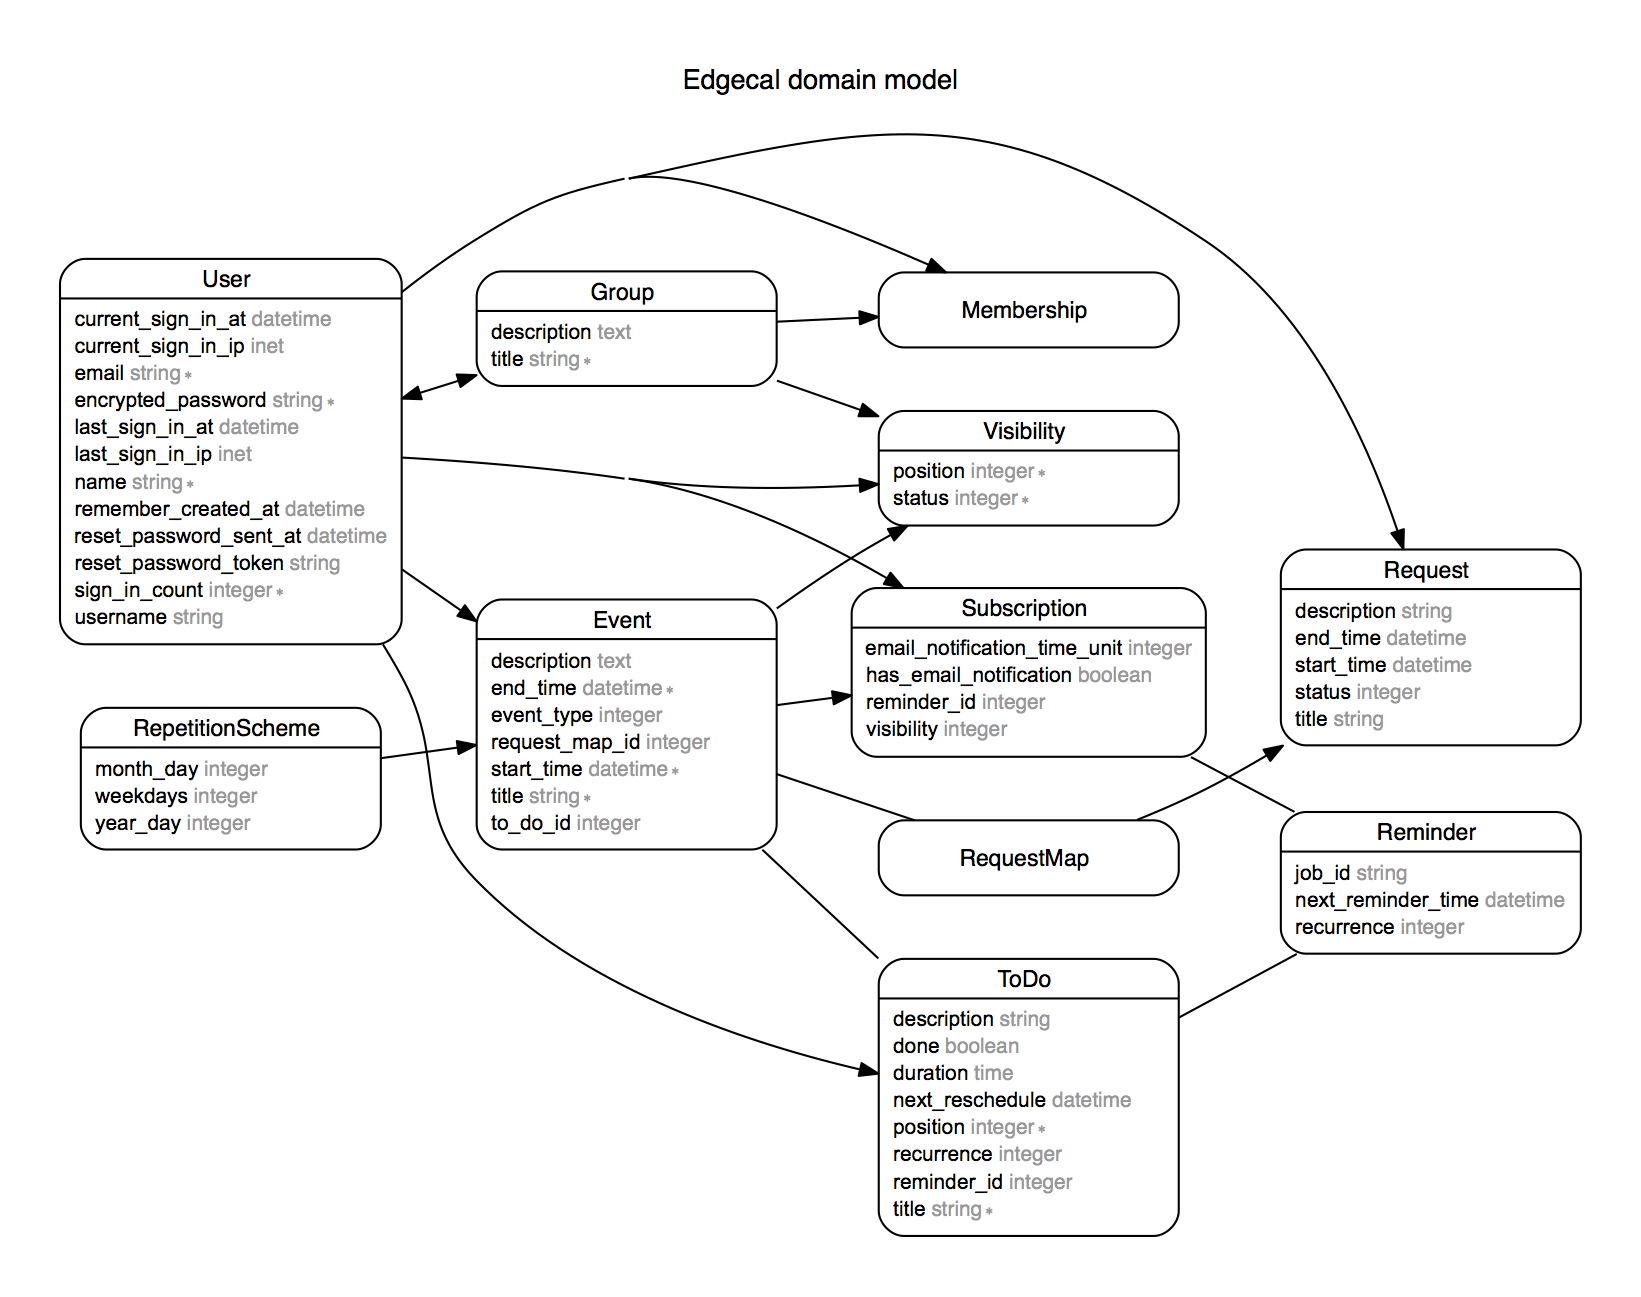
\includegraphics[scale=0.6]{erd.png}
\caption{Database ERD Diagram}
\end{figure}

\begin{itemize}

  \item User: holds user general information along with the current session. A user has many created events and subscriptions to other user created events. It holds many memberships to groups defined by other users and many self-created to-dos. It also has many visibilities applied to him specifically regarding someone else’s event and several requests made by another person to him. A user model is responsible for retrieving any type of event with a certain characteristic related to him. Also, it creates and removes its own subscription.
  \item Event: Holds the general information of an event. It belongs to a creator, which is a User model. It holds many subscriptions made by other users to it and has many possible visibilities applied to it. It contains one to-do in case it is a to-do event or one request\_map in case it is a requested event. A column event\_type helps discern what type of event we are dealing with so we can present and consider it properly. We thought this design would be better rather than creating several event tables for each type and querying different tables to get essentially the same object. We let the event set itself up depending on its type. For instance, when a to-do event is created, it takes care of setting its title and description automatically based on the fetched to-do. Right now, the three possible types are ‘regular’, ‘to\_do’, and ‘request’.
  \item Group: represents a group with a name to which one can assign several members for organization. A group is linked to many memberships as it is a many-to-many relationship with Users. A group also has many visibilities as a visibility rule of an event can be assigned to whole groups.
  \item Membership: table that maps the many-to-many relationship between users and grops.
  \item Subscription: table that maps the many-to-many relationship between users and events. If the user has a subscription, the event will be displayed for him if the visibility is not private. A subscription also holds a reminder, so each user can set his own reminder to a specific event.
  \item Visibility: represents one visibility rule applied to one event by its creator. An event can have several visibilities and can have them ordered in whichever way the user wants. We make use of the act\_as\_list gem that orders the visibility by position, scopes unique values by its corresponding event, and rearranges all positions once one of the visibilities position is changed, allowing for always having a set of visibilities in a clearly defined order. A visibility can either belong to a user or group. We decided to not break a group in its members and assign several visibilities because if a user would try to move the position of a whole group visibility, it would be hard to keep track of the new position of each member that pertains to that group. We make use of enums mapped directly to a status column to discern the different visibilities.
  \item RequestMap: is basically a modularization level to manage the requests for an event. This way, an event that is not a request does not need to carry unnecessary behavior or information besides a request\_map\_id. It holds the relation to its many requests and is able to retrieve requests by status and create new ones for a given set of users.
  \item Request: model that most importantly holds a state for the views and controllers to handle the behavior of a user towards an event. A request holds its corresponding request\_map and user, and contains a status column to discern whether it is pending, confirmed, declined, removed, or with a requested modification.
  \item ToDo: is an asynchronous model that can be optionally embedded in an event. Much like a visibility, it also makes use of the acts\_as\_list gem to order the to-dos of a user by priority in a cohesive manner. If a to-do event is allocated, it automatically fetches the next to-do on the priority list that is not done and is not assigned to another event already. It holds its own creator id and has a column to define its optional recurrence. After the event gets done, it verifies if the recurrence time has elapsed since creation. If so, it immediately creates a new to-do with the same parameters. If not, it schedules the creation of another to-do to the proper time. It contains an optional reminder as well with recurrent characteristics.
  \item Reminder: Handles email notifications for either a subscription or a to-do. After creation, it schedules the right reminder based on the presence of a foreign key to either object. It holds a start\_time and a recurrence value for the initial and subsequent notifications. For scheduling, we use the rufus\_scheduler ruby gem.

\end{itemize}

\section{Future Design Needs}

\section{Design Process Notes}

This section of the document describes experiences regarding the design and testing process for each member of the team.  These experiences include analyzing data, design processes, and team management.

\subsection{Designed and Conducted Experiment}

\textit{Brian's Contribution}

One of the major components that I worked on during this evolution was getting our Calendar User Interface for viewing events fleshed out. One of the issues we ran into with Evolution 1 was with how our assets were served on our production server. Ruby on Rails leverages a resource called the Asset Pipeline which really does a lot for the developer. It allows you to write stylesheets and scripts in interpreted languages like Sass and Coffeescript, and it allows you to write multiple independent files that will later get concatenated together when deployed in production. It also performs asset fingerprinting to help with caching and compresses/minifies CSS and Javascript to further help with efficiency. One of the pain points with the Asset Pipeline, however, is that there are a few major differences between running in Development and running on Production. For example, in the production environment Rails pre-compiles and concatenates all of the CSS and Javascript. This can cause lots of syntax errors with missing semi-colons at the end of files, dependency ordering, and other issues. This ended up hurting us during Evolution 1 because we were working pretty much exclusively in our development environment, and only tried moving to production towards the very end. This caused our styling to get a little wacky on Heroku and the Calendar would not show up. 

Therefore for the first few days after Evolution 1 was finished up, I spent a lot of time researching the asset pipeline, and started designing tests and experiments to narrow down the problems. I was able to fix all of the syntax in the stylesheets, identified broken imports and scripts, and reconfigured some of the Gems to be consistent with the rest of our application. One of the key issues with the calendar UI we were using was with an inconsistency with the version of Ruby on the production and development servers. After many, many hours of researching, debugging, and fiddling, I was able to narrow down the problem to the Ruby version, and it instantly fixed our bug. 

\textit{Jeff's Contribution}

One key front end aspect that we wanted to add to our web application in Evolution 2 was popup forms and views.  As a team, we agreed that these types of views would not only would to a more fluid user experience, but generally look more modern.  In order to implement these popup forms (along with other various UI features), we added a Rails Gemfile called Foundation.  This Gemfile allows for easy inclusion of many jQuery elements in the views files of our Rails app.  Using an aspect of Foundation called reveal-modal, I attempted to implement the form to create a new group into a popup window that would allow the user to create a new group without leaving the index page.  I created the form and could submit without error, however the users were not being added to the group in the actual database.  After, attempting to modifying aspects of the reveal-modal, I instead tried implementing my new group form in a simple rails view page instead of attempting to add dynamic popup views.  When trying a normal form and realizing that the database was successfully populated with that form, it was obvious that the issue was with submitting data using reveal-modal.  After more research, it became obvious that to do form submittal in a popup view, we need to utilize AJAX with dynamic page loading.

\textit{Wes's Contribution}

After creating the mailers folder and configuring an email message that I wanted to have sent to users, I needed to figure out exactly how the email was going to be sent, and whether it would be sent at the right time.  Our group installed a rails gem called rufus-scheduler that makes it easy to schedule tasks for certain times, and then as long as the server and database is still running, it will wake up and run those tasks.  However, when I first configured the mailers, no emails were being sent.  Since we are using an app called Mailgun for our email domain, I was able to look at the logs and see that the scheduler wasn’t waking up at all, and therefore wasn’t running the method that sent emails.  I placed “puts” statements in the few methods that were most related to the mailers, and tried to see where the code was going wrong.  After narrowing it down to the method that creates our Rufus scheduler, I determined that even though the “puts” statement right before our email method was run with the proper information, there was a typo in the line that actually ran the method which did not give us an error when run.  This entire process took a long time to debug, and the typo was not a trivial typo to pick up on unless you had written the method, which I had not.  However, I was able to eventually figure it out, and correct the error.

\subsection{Analyzed and Interpreted Data}

\textit{Brian's Contribution}

One of the vital components of Web applications is the passing and handling of data. To do this you need to understand the basic RESTful HTTP methods, how routing works (specific to your framework), and some useful data formats like JSON. In this evolution I ended up working heavily with passing data to components beyond the basic CRUD methods in the controllers that Rails sets up for you. After learning all about this, I was able to structure custom RESTful calls to pass JSON data to the front-end calendar UI as well as pass different data and parameters to pop-up Modals and other non-standard views. This would not have been possible without significant testing. By logging all of the server calls and parsing through the HTML requests I was able to identify exactly how and where requests were being sent and was able to diagnose issues much more quickly. 

\textit{Jeff's Contribution}

Throughout our teams development in the Rails framework, the ability to read and understand messages outputted from the rails server has become incredibly important, specifically with debugging.  My previously mentioned bug involved not only designing an experiment, but also interpreting specific terminal data in order to successfully debug.  The specific issue was that the checkboxes associated with the form were not being properly read by Rails as a result of being in the reveal-modal window.  With functioning checkboxes, the successful creation of a group results in the terminal outputting a visualization of a map associating the id of each user with a one or zero (representing whether they were added to the group or not).  Originally I did not realize that this was the desired terminal output; I only new that the terminal was outputting that the addition of users to the groups members column was forbidden.  However, after reviewing the output of a similar form that Henrique had implemented, I was able to see what the correct output should look like and deduce that the issue was with Foundation, not my implementation of the form.  Only through the ability to understand and analyze this sort of server data was I able to completely debug this issue.

\textit{Wes's Contribution}

When our group was implementing the rufus-scheduler in our project, we needed to be sure that the time zone of the user was taken account of when they set reminders for themselves.  Since our database stores all information in UTC time, reminders were stored five hours ahead of when they would actually be woken up for Eastern Time.  To ensure this, we wrote a method called start_time_makes_sense in the reminder model, which uses “puts” to print the current time next to the time being stored, and then makes sure that the reminder is not before the current time (in which case it would never happen).  We also compared this data to the data being stored in our database, which made sure that the time was being properly converted to UTC time, which should be five hours ahead of Eastern Time.

\subsection{Designed System Component to Meet Desired Needs}

\textit{Brian's Contribution}



\textit{Jeff's Contribution}

\textit{Wes's Contribution}

In designing the mailer, I had to interact a lot with the models and controllers that deal with PUDs and subscriptions.  In our model, a “subscription” is any relationship between a user and an event.  For example, a user may have an owner subscription to an event, meaning he/she created that event and has full permission to edit/delete it.  A user may also only have a visible subscription to an event, meaning they can see an event, but cannot change it.  This subscription model made it much easier to handle the email reminder process, since each subscription only relates one user to one event, and can therefore have a reminder email embedded in it if a user wants to be reminded of something.  The reminder model is where the rufus-scheduler is run, so we can effectively schedule any kind of reminder we want as soon as a subscription is made.  We can also leave the reminder form blank, in which case there will be no email notification for a subscription.  By creating our email reminders in this way, it should be easy to further customize email notifications in our project.

\subsection{Deal with Realistic Constraints}

\textit{Brian's Contribution}

As usual, the front-end embellishments became less of a priority on this evolution. While we were very happy with how well how model was able to be extended to meet the new requirements, we still had to do a lot of work to get the basic functionality up and running. While we hoped that we could have added a lot more dynamic content with JQuery and AJAX, it became a much lower priority as the project went on and reality set in. A few of the minor bugs with some corner cases on form submission and in other places also were not entirely fleshed out until very late in the process. From what we have seen and experimented with, most of these issues have been worked out, but due to time constraints we were unable to develop robust tests to ensure the robustness of our application.

\textit{Jeff's Contribution}

As always with large scale CS projects as an undergraduate, my team was constrained by time towards the end of evolution two work period, especially as a result of other midterms and big assignments due among the team.  As a result of this fact, we had to ignore some smaller bugs in order to work on other more significant ones.  For example, one of my jobs towards the end of the evolution period was to discover why our calendar would only render after going to the main events page and then refreshing.  However, at that point in time, we still did not have recurring events working completely.  At that point, Henrique and I decided that it was more important for me to assist him with developing methods to make recurring event creation easier than it was to make the calendar render on every event page click.

\textit{Wes's Contribution}

Our team really wanted to try and incorporate more dynamic content into our website for this evolution; things like modals forms, popup alerts, color coordinated alert messages, etc.  However, these additions require a decent amount of knowledge of JavaScript, JQuery, or AJAX, to name a few of the possibilities.  As we continued to progress on our project, these embellishments took a back seat to functionality, and we actually found out that many of the forms that were very intuitive in the Rails framework were much more complicated to implement in some form of JavaScript.  In light of this, we decided to scrap many of our ideas for dynamic content and work more on ensuring our static content worked the way it should.  I think this is something we can definitely work on for the next evolution as we seek to streamline the user experience on our website. 

\subsection{Contributed to Team Work and Interacted with Team Members}

\textit{Brian's Contribution}



\textit{Jeff's Contribution}

There were two primary tracks for interacting with my team members: through project management tools and in person.  Using tools like Trello, Facebook Chat, and useful commit comments, I did my best to always keep the rest of the team updated on how progress on my responsibilities was going.  This not only allowed team members to assist me if they saw any flaws in the work I was doing, but also just kept the entire team on the same page.  Throughout this evolution, the primary way that my team and I worked well as a team in person was through pair programming and peer code reviews.  Often if one of us had an issue with some aspect of the project, a fresh pair of eyes or a new way of thinking about some specific algorithm quickly solved the problem.  This sort of team interaction not only allowed me to help my teammates, but also allowed the to help me in a very effective manner.

\textit{Wes's Contribution}

Our group was experiencing some very persistent errors when trying to migrate our more recent work to our production server run on Heroku.  For whatever reason, the dynamic content that used JavaScript was not running at all, which crippled some functionality we had spent a lot of time creating.  Brian spent a HUGE chunk of time testing our app to see where this error could be occurring, but for two days had not had much success.  He and I decided to do some work next to each other one night, and as I was working on my part of the project, I would randomly come up with a few reasons why I thought the production server wasn’t running.  One of these reasons, that our version of Ruby or Rails was not consistent in our development and production environments, ended up being the actual bug.  I suggested this to Brian, and we were elated that it ended up working after forcing Ruby to run version 2.2.0 in our production server.  Brian and I spent the better part of a night trying to find this bug, and we were obviously frustrated that it was something so simple, but also happy that we had figured it out.


\end{document}